\documentclass[a4paper, twocolumn]{article}


% you can switch between these two (and more) styles by commenting one out (use percentage)
\usepackage[backend=biber]{biblatex}
%\usepackage[backend=biber, style=authoryear-icomp]{biblatex}
\addbibresource{./refs.bib}

\usepackage{graphicx}

\usepackage{listings}
\usepackage{color}
\definecolor{lightgray}{gray}{0.9}

% code listing: https://tex.stackexchange.com/questions/19004/how-to-format-an-inline-source-code
\lstset{
    showstringspaces=false,
    basicstyle=\ttfamily,
    keywordstyle={blue},
    commentstyle=\color[gray]{0.6}
    stringstyle=\color[RGB]{255, 150, 75}
}
\newcommand{\inlinecode}[2]{\colorbox{lightgray}{\lstinline[language=#1]$#2$}}

\author{Henrik Strøm}
\title{Using \LaTeX}



\begin{document}

\twocolumn[
    \begin{@twocolumnfalse}
        \maketitle
        \begin{abstract}
            LaTeX is an extremely powerful typesetting system.
            This document demonstrates some basic usage.
        \end{abstract}
    \end{@twocolumnfalse}
    \vspace{1cm}
]


\section{Introduction\label{sec:Introduction}}
According to \cite{example_website}, ...

Lorem ipsum dolor sit amet, consectetur adipiscing elit, sed do eiusmod tempor incididunt ut labore et dolore magna aliqua. Ut enim ad minim veniam, quis nostrud exercitation ullamco laboris nisi ut aliquip ex ea commodo consequat. Duis aute irure dolor in reprehenderit in voluptate velit esse cillum dolore eu fugiat nulla pariatur. Excepteur sint occaecat cupidatat non proident, sunt in culpa qui officia deserunt mollit anim id est laborum.

Here is a reference to a scientific paper, you can find it in the references.
\cite{lecun1995convolutional}
You can do it like this, e.g., if you want to talk about the paper by
\textcite{lecun1995convolutional}
You can also use
\parencite{lecun1995convolutional}


Paragraphs are separated by empty lines.
It might be a good idea to put every sentence on a separate line -- that way \inlinecode{bash}{git} will work on a sentence-by-sentence basis.

\section{Formatting in \LaTeX\label{sec:Formatting in Latex}}


\subsection{Lists}
\label{sec:Lists}

You can make nice lists in \LaTeX:

\begin{itemize}
    \item First item
    \item Second item
\end{itemize}

Or like this:

\begin{enumerate}
    \item First item
        \begin{enumerate}
            \item Sub element
        \end{enumerate}
    \item Second item
        \begin{itemize}
            \item Another sub element
        \end{itemize}
\end{enumerate}


\subsection{Text Decoration\label{sec:Text Decoration}}


Different text decorations like \textit{textit}, \emph{emph} (which might render differently than here), \textbf{textbf} are possible, and it might be a good idea to find a \LaTeX cheat-sheet to find out more.

You can put things in quotes like "Hey, look at that!", or ``Hey, look at that!''.
Notice these are not identical.


\subsection{Quoteblocks\label{sec:Quoteblock}}

Quote blocks look nice:

\begin{quote}
\emph{
I believe that in about fifty years' time it will be possible, to programme computers (..) to make them play the imitation game so well that an average interrogator will not have more than 70 per cent chance of making the right identification after five minutes of questioning.
}
\cite{turing1950computing}
\end{quote}


\subsection{Tables\label{sec:Tables}}

Things like tables are obviously supported in \LaTeX, see table \ref{table:Likert scale and scoring}.

\begin{table}[ht]
    \caption{Likert scale and scoring}
    \centering
    \begin{tabular}{r | l}
        \hline\hline
        Score & Answer \\ [0.5ex] % inserts table %heading
        \hline
        -2 & Strongly disagree \\
        -1 & Disagree to some extent \\
        1 & Agree to some extent \\
        2 & Strongly agree \\ [1ex]
        \hline
    \end{tabular}
    \label{table:Likert scale and scoring}
\end{table}


\subsection{Equations\label{sec:Equations}}

The cost function we most often use in classification is shown in Equation \ref{eq:cost-function-classification}.

\begin{equation}
    \label{eq:cost-function-classification}
    J_\theta(X) = -\frac{1}{m} \sum (Y \cdot log(h_\theta(X)) + (1 - Y) \cdot log(1 - h_\theta(X))
\end{equation}


\subsection{Figures\label{sec:figures}}

Figure \ref{fig:univariate-linear-fit-cost} shows the reduced cost over number of iterations running batch gradient descent.

\begin{figure}[h]
    \centering
    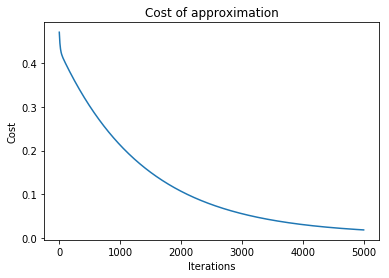
\includegraphics[width=0.5\textwidth]{figures/univariate-linear-fit-cost.png}
    \caption{Reduction of the cost function over iterations.}
    \label{fig:univariate-linear-fit-cost}
\end{figure}


\printbibliography

\end{document}

